\section{Pendahuluan}
\subsection{Latar Belakang}
Di era digital saat ini, jaringan komputer memainkan peran vital sebagai sarana utama dalam komunikasi dan pertukaran data. Untuk menciptakan jaringan yang stabil dan terpercaya, diperlukan pemahaman yang menyeluruh mengenai teknik penyambungan kabel (crimping) serta pengelolaan alamat jaringan (routing IPv4). Crimping merupakan metode penyambungan kabel tembaga, seperti kabel UTP (Unshielded Twisted Pair), dengan konektor RJ45 untuk menghasilkan kabel jaringan yang siap digunakan. Teknik ini sangat penting guna memastikan hubungan fisik yang andal dan efisien dalam jaringan lokal (LAN). Di sisi lain, routing IPv4 adalah proses pengiriman data antar perangkat dalam jaringan dengan memanfaatkan alamat IP versi 4, yang hingga kini masih menjadi standar umum dalam berbagai sistem jaringan. Pengetahuan tentang crimping dan routing IPv4 menjadi hal yang krusial bagi para teknisi jaringan, khususnya dalam proses perancangan, penerapan, dan pemeliharaan infrastruktur jaringan komputer. Penerapan teknik crimping yang tepat dapat mengurangi gangguan sinyal serta meningkatkan kinerja jaringan, sementara manajemen routing yang baik menjamin data dapat dikirim dengan cepat dan tepat sasaran. Laporan ini disusun untuk membahas dasar-dasar dari crimping dan routing IPv4 sebagai landasan awal dalam mempelajari teknologi jaringan lebih lanjut.

\subsection{Dasar Teori}
\subsection*{Crimping}
Crimping adalah proses menyambungkan kabel jaringan, terutama kabel UTP, ke konektor RJ45 menggunakan alat khusus yang disebut crimping tool. Kabel UTP sendiri terdiri dari empat pasang kawat tembaga yang dipilin untuk meminimalisir gangguan elektromagnetik. Saat melakukan crimping, penting untuk menyusun urutan warna kabel sesuai standar tertentu, seperti T568-A atau T568-B, tergantung jenis koneksi yang diinginkan. Misalnya, kabel straight-through digunakan untuk menghubungkan perangkat berbeda seperti komputer ke switch atau router, di mana urutan kabel di kedua ujungnya sama. Sedangkan kabel crossover digunakan untuk menyambungkan perangkat yang sejenis, seperti antara dua komputer atau dua switch, dengan susunan warna yang berbeda di salah satu ujungnya.Langkah-langkah crimping dimulai dengan mengupas bagian luar kabel UTP untuk menampakkan kawat tembaganya, lalu menyusunnya sesuai urutan warna standar. Setelah itu, kawat-kawat tersebut dimasukkan ke dalam konektor RJ45 hingga ujungnya menyentuh bagian dalam konektor. Proses ini diakhiri dengan menekan konektor menggunakan crimping tool agar pin di dalamnya mencengkeram kawat tembaga dengan kuat. Untuk memastikan hasilnya baik, kabel yang sudah dicrimping sebaiknya diuji dengan cable tester guna mengecek apakah semua sambungan telah terhubung dengan benar dan tidak ada koneksi yang terputus.
\subsection*{Routing IPv4}
Routing IPv4 adalah proses mengirimkan data antarjaringan berdasarkan alamat IP tujuan. Protokol IPv4 menggunakan alamat 32-bit yang ditulis dalam format desimal bertitik, seperti 192.168.1.1, dan terdiri dari dua bagian: Network ID yang menunjukkan lokasi jaringan, dan Host ID yang mengidentifikasi perangkat di dalam jaringan tersebut. Proses routing dilakukan oleh perangkat jaringan seperti router yang menentukan jalur pengiriman data dengan mengacu pada tabel routing. Tabel ini menyimpan informasi penting seperti alamat tujuan, gateway, dan metrik untuk menentukan rute terbaik.Terdapat dua jenis utama routing, yaitu static routing dan dynamic routing. Pada static routing, administrator jaringan secara manual menentukan jalur pengiriman data. Cara ini lebih cocok untuk jaringan kecil yang jarang berubah. Sementara itu, dynamic routing memungkinkan router untuk secara otomatis memperbarui jalur dengan menggunakan protokol seperti RIP, OSPF, atau BGP, yang lebih efektif untuk jaringan yang besar dan kompleks.Selain itu, konsep subnetting juga sangat penting dalam manajemen jaringan. Teknik ini membagi jaringan besar menjadi beberapa jaringan kecil (subnet) agar lebih efisien dan aman. Subnetting menggunakan subnet mask, misalnya 255.255.255.0, untuk memisahkan bagian Network ID dan Host ID dalam sebuah alamat IP. Sebagai contoh, alamat 192.168.1.10 dengan subnet mask tersebut menunjukkan bahwa 24 bit pertama adalah bagian dari Network ID, sementara 8 bit sisanya adalah Host ID.Dengan memahami crimping dan routing IPv4, kita dapat membangun jaringan yang tidak hanya kuat secara fisik, tetapi juga optimal dalam mengelola arus data di dalamnya.

%===========================================================%
\section*{Tugas Pendahuluan}
\begin{enumerate}
    \item \textbf{Alokasi IP Tiap Departemen}

    Setiap departemen dalam jaringan perusahaan memiliki jumlah perangkat yang berbeda, sehingga alokasi alamat IP disesuaikan dengan kebutuhan masing-masing. Departemen Produksi, dengan 50 perangkat, memerlukan minimal 64 alamat IP agar mencakup juga alamat jaringan dan broadcast. Oleh karena itu, digunakan prefix \texttt{/26} yang menyediakan 64 alamat dalam rentang 0--63.

    Untuk Departemen Administrasi yang memiliki 20 perangkat, dibutuhkan setidaknya 32 alamat IP. Maka digunakan prefix \texttt{/27}, dengan rentang alamat 64--95. Departemen Keuangan, yang terdiri dari 10 perangkat, memerlukan 16 alamat dan menggunakan prefix \texttt{/28} dengan rentang 96--111.

    Terakhir, Departemen R\&D memiliki kebutuhan terbesar, yaitu 100 perangkat. Oleh karena itu dialokasikan prefix \texttt{/25} yang mencakup 128 alamat IP, dengan rentang 128--255.

    \item \textbf{Topologi Jaringan}

    Topologi jaringan yang digunakan adalah \textit{star topology}, di mana satu router utama menjadi pusat koneksi yang menghubungkan keempat subnet dari masing-masing departemen. Masing-masing departemen dihubungkan ke router melalui antarmuka yang berbeda, menggunakan \textit{switch} lokal.

    \begin{figure}[H]
        \centering
        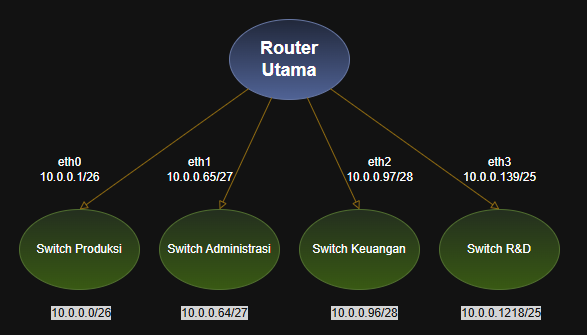
\includegraphics[width=0.5\linewidth]{Screenshot 2025-05-09 135115.png}
        \label{fig:enter-label}
    \end{figure}

    \textit Diagram di atas memperlihatkan koneksi antara router utama dan masing-masing \textit{switch} departemen. Setiap antarmuka router (eth0 hingga eth3) terhubung ke subnet tertentu, sesuai alokasi IP yang telah direncanakan.

    \item \textbf{Tabel Routing}
    Router utama memerlukan tabel routing untuk mengarahkan lalu lintas data antar subnet. Berikut adalah tabel yang digunakan:
    \begin{table}[h]
    \centering
    \renewcommand{\arraystretch}{1.3}
    \begin{tabular}{|c|c|c|c|}
    \hline
    \textbf{Network Destination} & \textbf{Netmask / Prefix} & \textbf{Gateway} & \textbf{Interface} \\ \hline
    10.0.0.0 & 255.255.255.192 /26 & 10.0.0.1 & eth0 \\ \hline
    10.0.0.64 & 255.255.255.224 /27 & 10.0.0.65 & eth1 \\ \hline
    10.0.0.96 & 255.255.255.240 /28 & 10.0.0.97 & eth2 \\ \hline
    10.0.0.128 & 255.255.255.128 /25 & 10.0.0.129 & eth3 \\ \hline
    \end{tabular}
    \end{table}

    \textit{Penjelasan:} Tabel di atas menunjukkan bahwa setiap subnet dihubungkan langsung ke antarmuka router. Alamat gateway merepresentasikan IP antarmuka router di masing-masing subnet, sementara kolom prefix menunjukkan ukuran alokasi jaringan berdasarkan jumlah host yang dibutuhkan.

    \item \textbf{Jenis Routing yang Digunakan}

    Berdasarkan ukuran dan skala jaringan yang hanya mencakup sekitar 180 perangkat dengan empat LAN, jenis routing yang paling tepat digunakan adalah \textit{static routing}. Konfigurasi ini cukup efisien dan mudah dikelola untuk jaringan berskala kecil hingga menengah. Namun, agar alokasi alamat IP lebih optimal dan fleksibel, penggunaan teknik CIDR (Classless Inter-Domain Routing) sangat dianjurkan.
\end{enumerate}